\section{Results}\label{sec:results}

\subsection{Single-Qubit Operations and Bell State Entanglement}
\label{subsec:single-qubit-bell}

Applying the Pauli operators defined in \cref{section:methods} confirms the expected behaviour.

\begin{flalign}
\sigma_x \ket{0} &= \ket{1} & \sigma_x \ket{1} &= \ket{0} && \text{bit-flip} \\
\sigma_y \ket{0} &= i\ket{1} & \sigma_y \ket{1} &= -i\ket{0} && \text{bit-flip + phase} \\
\sigma_z \ket{0} &= \ket{0} & \sigma_z \ket{1} &= -\ket{1} && \text{phase-flip}
\end{flalign}

The Hadamard gate (H) maps computational basis states to equal superpositions, $H\ket{0}=\ket{+}$ and $H\ket{1}=\ket{-}$. The phase gate introduces a relative phase of $i$ on $\ket{1}$ while leaving $\ket{0}$ unchanged. In our results, both gates act as expected. 
\begin{figure}[!htbp]
    \centering
    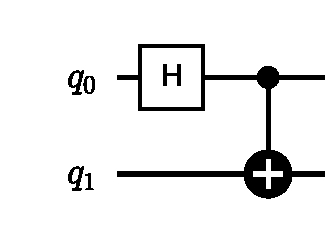
\includegraphics[width=0.55\linewidth]{figures/circuit_bell_state.pdf}
    \caption{Quantum circuit for the preparation of the Bell state $\ket{\Phi^+}$. The two qubits are initialized in the $\ket{00}$ state. A Hadamard gate ($H$) is applied to the first qubit, creating a superposition state. This is followed by a CNOT gate with the first qubit as the control and the second as the target, creating the maximally entangled state $\frac{1}{\sqrt{2}}(\ket{00} + \ket{11})$}
    \label{fig:circuit-bell-state}
\end{figure}
Starting from $\ket{00}$, the circuit $H\otimes\textbf{I}$ followed by CNOT produced \cref{h-otimes-I-cnot}, illustrated in \cref{fig:circuit-bell-state}, and with repeated measurement of $\ket{\Phi^+}$ with $50$ runs times $1000$ shots yielded the table seen in \cref{tab:measurement-probabilities}.
\begin{equation}\label{h-otimes-I-cnot}
\ket{00} 
\xrightarrow{H\otimes\textbf{I}} 
\frac{1}{\sqrt{2}}\left(\ket{00}+\ket{10}\right)
\xrightarrow{\text{CNOT}}
\frac{1}{\sqrt{2}}\left(\ket{00}+\ket{11}\right)
=
\ket{\Phi^+}
\end{equation}
\begin{table}[!htbp]
\centering
\begin{tabular}{ccc}
\hline
Outcome & $\mu$ & $\sigma$ \\
\hline
$\ket{00}$ & 0.4988 & 0.018 \\
$\ket{01}$ & 0.0000 & 0.000 \\
$\ket{10}$ & 0.0000 & 0.000 \\
$\ket{11}$ & 0.5012 & 0.018 \\
\hline
\end{tabular}
\caption{Mean measurement probabilities ($\mu$) and standard deviations ($\sigma$) obtained from repeated circuit evaluations.}
\label{tab:measurement-probabilities}
\end{table}

The outcomes are exclusively $\ket{00}$ and $\ket{11}$ with equal probability, which is the exact expected signature of the $\ket{\Phi^+}$ Bell state. The two qubits are perfectly correlated, measuring one immediately determines the other. The statistical fluctuations of $\sigma\approx0.018$ are consistent with the expected noise, as in \cref{expected-noise}
\begin{equation}\label{expected-noise}
    \sqrt{\frac{p(1-p)}{N_\text{shots}}}\approx0.016
\end{equation}
\begin{figure}[!htbp]
    \centering
    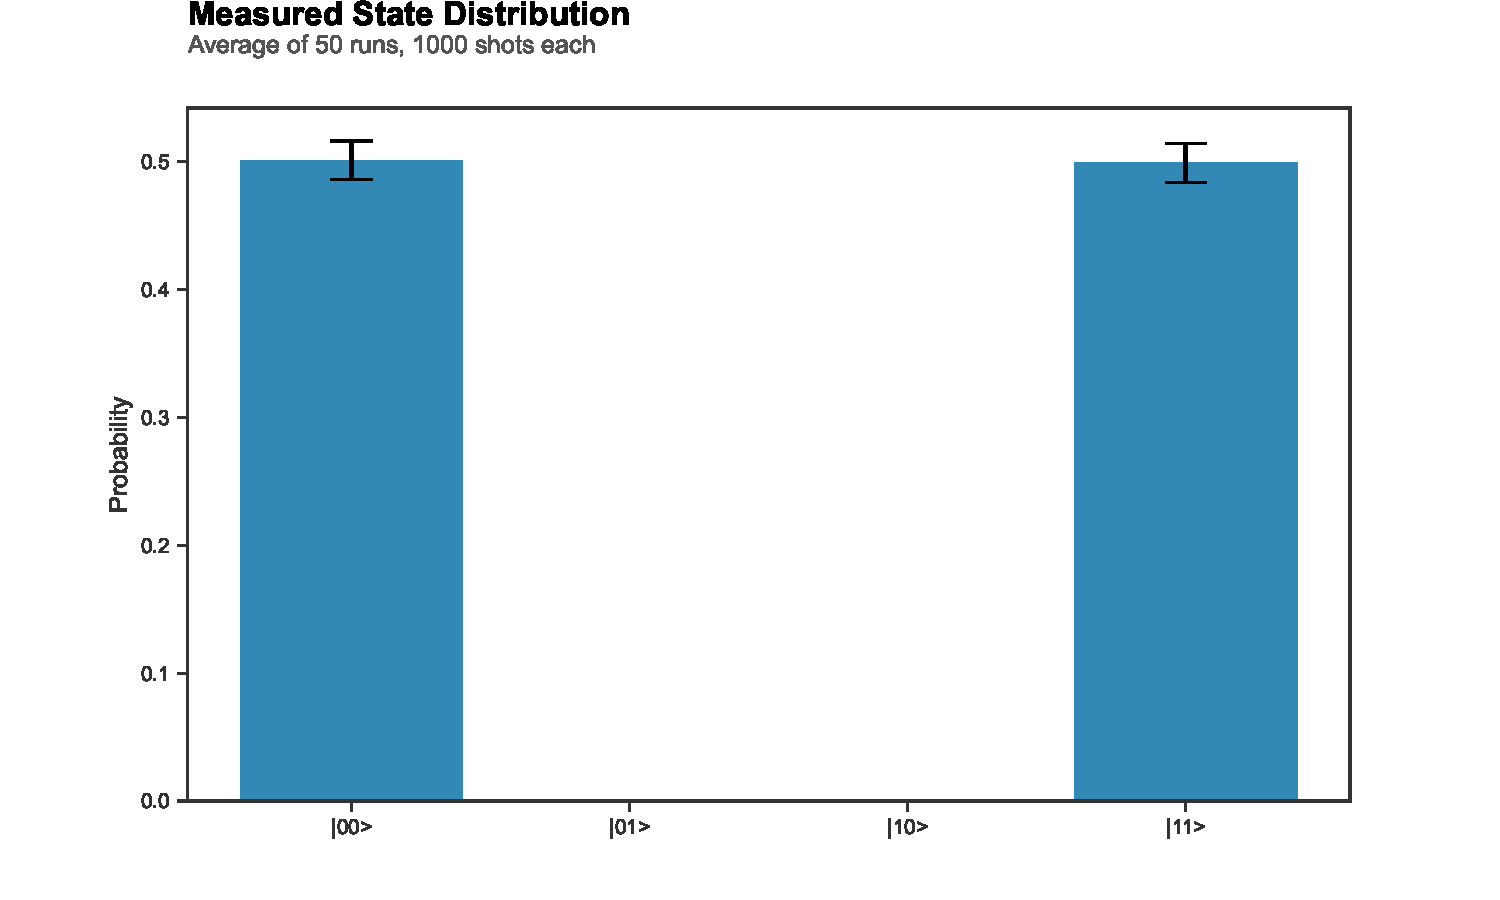
\includegraphics[width=\linewidth]{figures/part-a_measurement_dist.pdf}
    \caption{Measurement outcome distribution over 50 runs of 1000 shots each, showing near-equal probabilities for $\ket{00}$ and $\ket{11}$ as expected for the $\ket{\Phi^+}$ Bell state.}
    \label{fig:part-a_measurement_dist}
\end{figure}

Next, computing the von Neumann entropy $\mathcal{S}=-\text{Tr}\left(\rho_A\log_2\rho_A\right)$ in \cref{tab:entanglement-entropy-states}. 
\begin{table}[!htbp]
\centering
\begin{tabular}{lcc}
\hline
State & Type & $S$ \\
\hline
$\ket{\Phi^{+}}$ & Maximally entangled & 1.000 \\
$\ket{\Phi^{-}}$ & Maximally entangled & 1.000 \\
$\ket{\Psi^{+}}$ & Maximally entangled & 1.000 \\
$\ket{\Psi^{-}}$ & Maximally entangled & 1.000 \\
$\ket{00}$ & Product state & 0.000 \\
$\ket{+}\otimes\ket{0}$ & Product (superposition) & 0.000 \\
\hline
\end{tabular}
\caption{Von Neumann entropy $\mathcal{S}$ for several two-qubit states. The Bell states $\ket{\Phi^{\pm}}$ and $\ket{\Psi^{\pm}}$ are maximally entangled with $\mathcal{S}=1$, while product states have vanishing entropy.}
\label{tab:entanglement-entropy-states}
\end{table}

The entropy $\mathcal{S}=1$ bit for all four Bell states confirms they are maximally entangled: no local description of either qubit alone can capture the full state. Measuring one qubit instantly fixes the outcome of the other, regardless of the basis. For the product states $\ket{00}$ and $\ket{+}\otimes\ket{0}$, the entropy vanishes exactly. The superposition state $\ket{+}\otimes\ket{0}$ is instructive: even though qubit $A$ is in a superposition, the two qubits carry no correlations with each other, and the reduced density matrix of either subsystem is already pure. This underscores that von Neumann entropy measures entanglement, not superposition or classical uncertainty.

\subsection{Two-Level System: Exact Diagonalization vs.\ VQE}
\label{subsec:two-level-vqe}

Using parameters $E_1=0,\space E_2=4,\space V_{11}=3,\space V_{22}=-3,\space V_{12}=V_{21}=0.2$ the Pauli decompositions are shown in \cref{tab:pauli-decomposition-coefficients}.
\begin{table}[!htbp]
\centering
\begin{tabular}{lcc}
\hline
Coefficient & Value & Expression \\
\hline
$\mathcal{E}$ & $2.0$ & $\frac{E_1 + E_2}{2}$ \\
$\Omega$ & $-2.0$ & $\frac{E_1 - E_2}{2}$ \\
$c$ & $0.0$ & $\frac{V_{11} + V_{22}}{2}$ \\
$\omega_z$ & $3.0$ & $\frac{V_{11} - V_{22}}{2}$ \\
$\omega_x$ & $0.2$ & $V_{12}$ \\
\hline
\end{tabular}
\caption{Pauli decomposition coefficients from the project}
\label{tab:pauli-decomposition-coefficients}
\end{table}

The eigenvalues $E_\pm(\lambda)$ are computed both analytically and numerically (using \texttt{numpy.linalg.eigh}) over $101$ values of $\lambda\in[0,1]$, where the maximum discrepancy between the two methods are $\approx10^{-15}$, as shown in \cref{fig:part-b_eigenvalues}. 
\begin{figure}[!htbp]
    \centering
    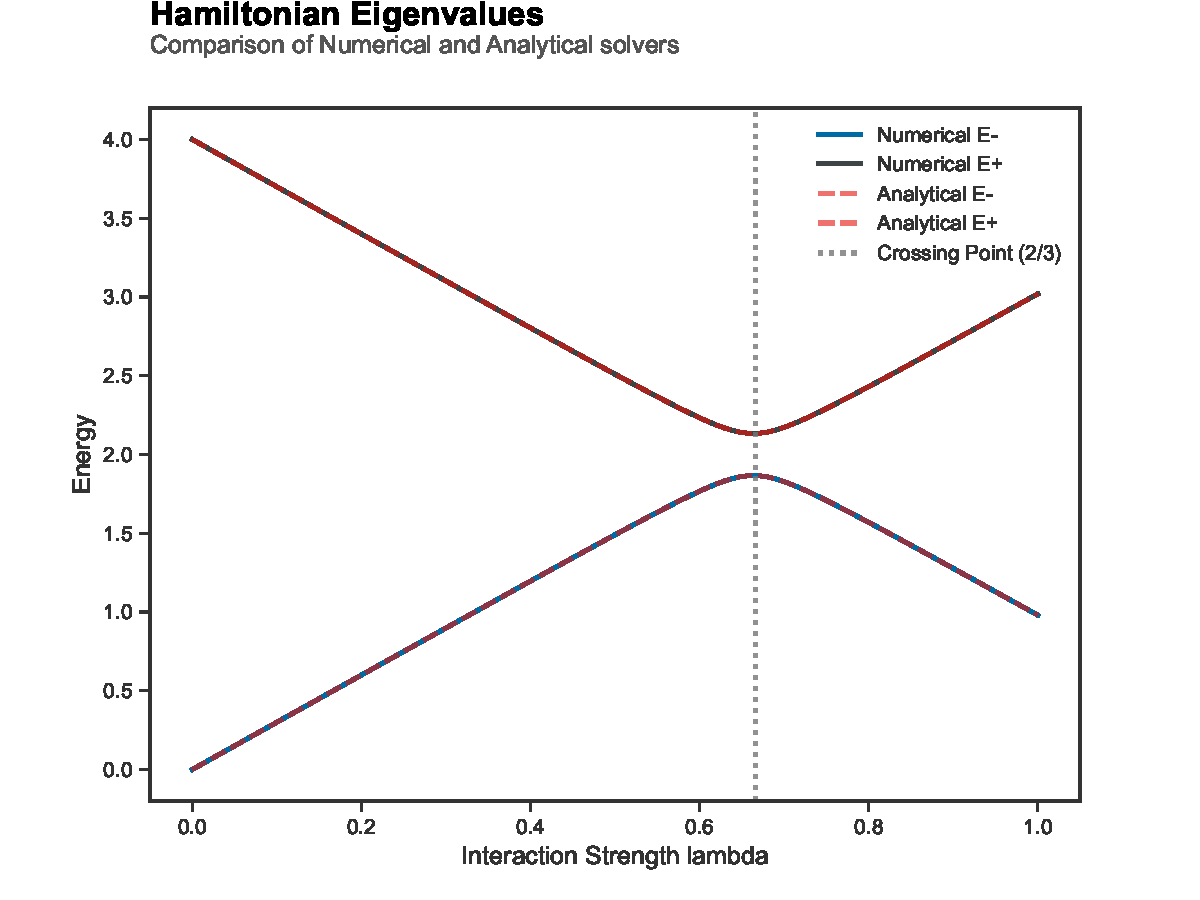
\includegraphics[width=\linewidth]{figures/part-b_eigenvalues.pdf}
    \caption{Eigenvalues $E_\pm(\lambda)$ as a function of the interaction parameter $\lambda$, obtained by both analytical and numerical diagonalization. An avoided crossing occurs at $\lambda=\frac{2}{3}$.}
    \label{fig:part-b_eigenvalues}
\end{figure}

The spectrum shows an avoided crossing at $\lambda=\frac{2}{3}$, where at this point, the diagonal matrix elements cross $\left(3\lambda=4-3\lambda\right)$, but the off-diagonal coupling $V_{12}=0.2$ prevents a true degeneracy, creating a gap of $\Delta E\approx0.27$. 

Tracking the eigenvector decomposition of the ground state as a function of $\lambda$, as seen in \cref{tab:lambda-probabilities}.
\begin{table}[!htbp]
\centering
\begin{tabular}{cccc}
\hline
$\lambda$ & $\mathrm{Prob}(\ket{0})$ & $\mathrm{Prob}(\ket{1})$ & Character \\
\hline
0.0   & 100\% & 0\%   & Pure $\ket{0}$ \\
$\tfrac{2}{3}$ & $\sim$50\% & $\sim$50\% & Maximally mixed \\
1.0   & $\sim$1\%  & $\sim$99\% & Dominated by $\ket{1}$ \\
\hline
\end{tabular}
\caption{Measurement probabilities of the computational basis states $\ket{0}$ and $\ket{1}$ as a function of the interaction parameter $\lambda$.}
\label{tab:lambda-probabilities}
\end{table}
\begin{figure}[!htbp]
    \centering
    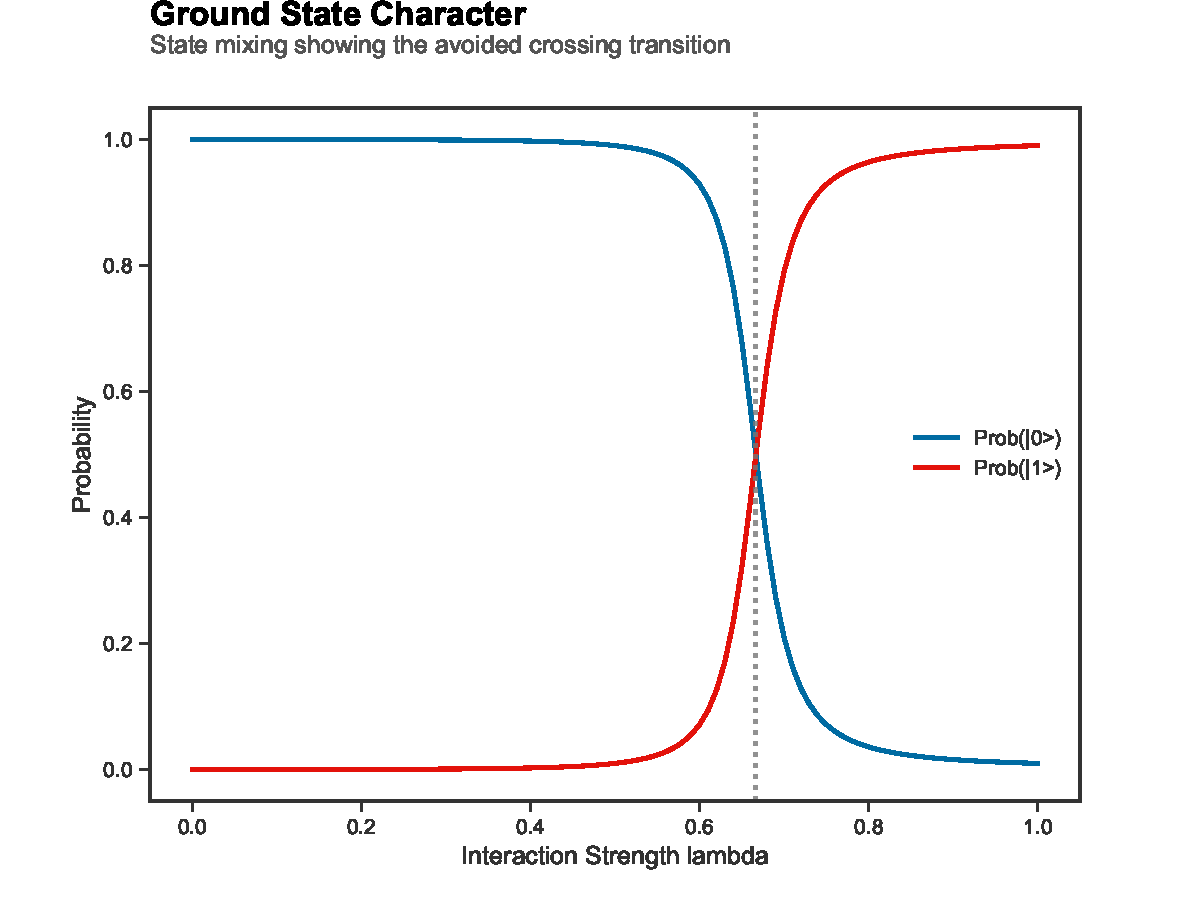
\includegraphics[width=\linewidth]{figures/part-b_eigenvector_mixing.pdf}
    \caption{Ground state character as a function of $\lambda$, showing the smooth transition from a $\ket{0}$-dominated state to a $\ket{1}$-dominated state through the avoided crossing.}
    \label{fig:part-b_eigenvector_mixing}
\end{figure}

The ground state character inverts as $\lambda$ passes through the crossing point. Below $\lambda=\frac{2}{3}$ it is predominantly $\ket{0}$, and above, $\ket{1}$ dominates. This transition is smooth because the coupling $V_{12}$ mixes the two basis states. At $\lambda=1$ only $\approx1\%$ of $\ket{0}$ remains, which is consistent with the theoretical prediction.

The trial state is shown in \cref{trial-state}, where the single-parameter rotation spans the full real single-qubit Hilbert space, since the Hamiltonian is real and symmetric, $R_y$ is exactly sufficient.
\begin{equation}\label{trial-state}
    \ket{\psi(\theta)} = R_y(\theta)\ket{0} = \cos\left(\frac{\theta}{2}\right)\ket{0}+\sin\left(\frac{\theta}{2}\right)\ket{1}
\end{equation}

The energy is evaluated as $E(\theta)=c_0+c_z\langle\sigma_z\rangle_\theta+c_x\langle\sigma_x\rangle_\theta$ where $\langle\sigma_z\rangle$ is obtained from computational-basis measurement and $\langle\sigma_x\rangle$ requires a Hadamard rotation before measurement. 

The VQE is swept over $\lambda\in[0,1]$. Both the ground state and the excited state accessed via $\theta_\text{opt}+\pi$ are computed. The VQE markers lie exactly on the exact diagonalization curves for both eigenvalues. Precision is shown in \cref{fig:part-c_vqe_spectrum_error} where the max error for the ground state is $5.41\times10^{-11}$ and excited state is same order.
\begin{figure}[!htbp]
    \centering
    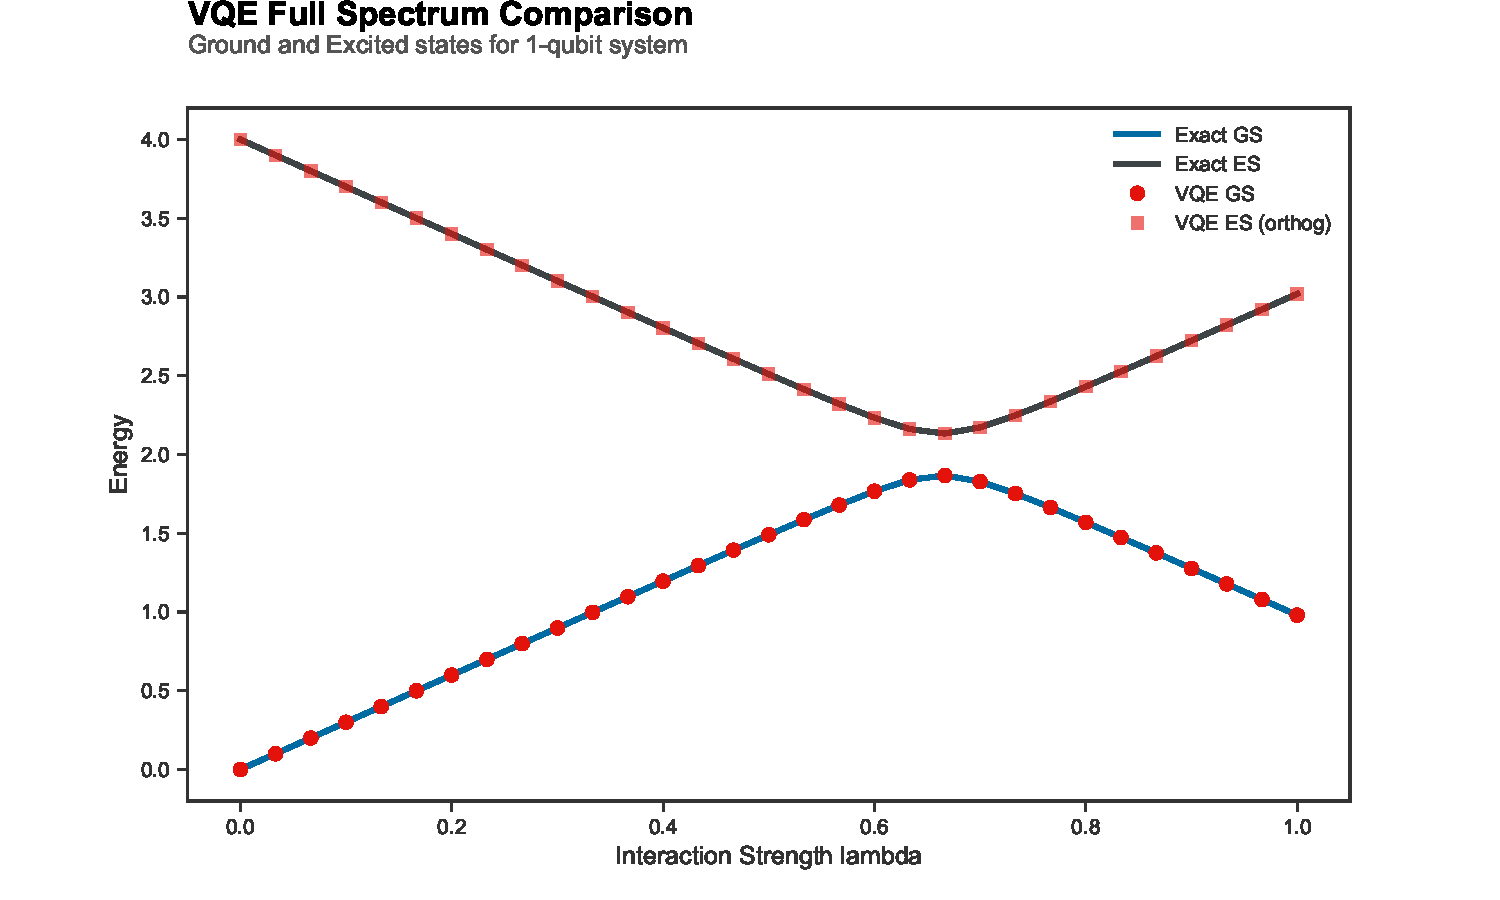
\includegraphics[width=\linewidth]{figures/part-c_vqe_full_spectrum.pdf}
    \caption{Full VQE spectrum showing both the ground state and excited state energies as a function of $\lambda$. VQE markers lie exactly on the exact diagonalization curves.}
    \label{fig:part-c_vqe_full_spectrum}
\end{figure}
\begin{figure}[!htbp]
    \centering
    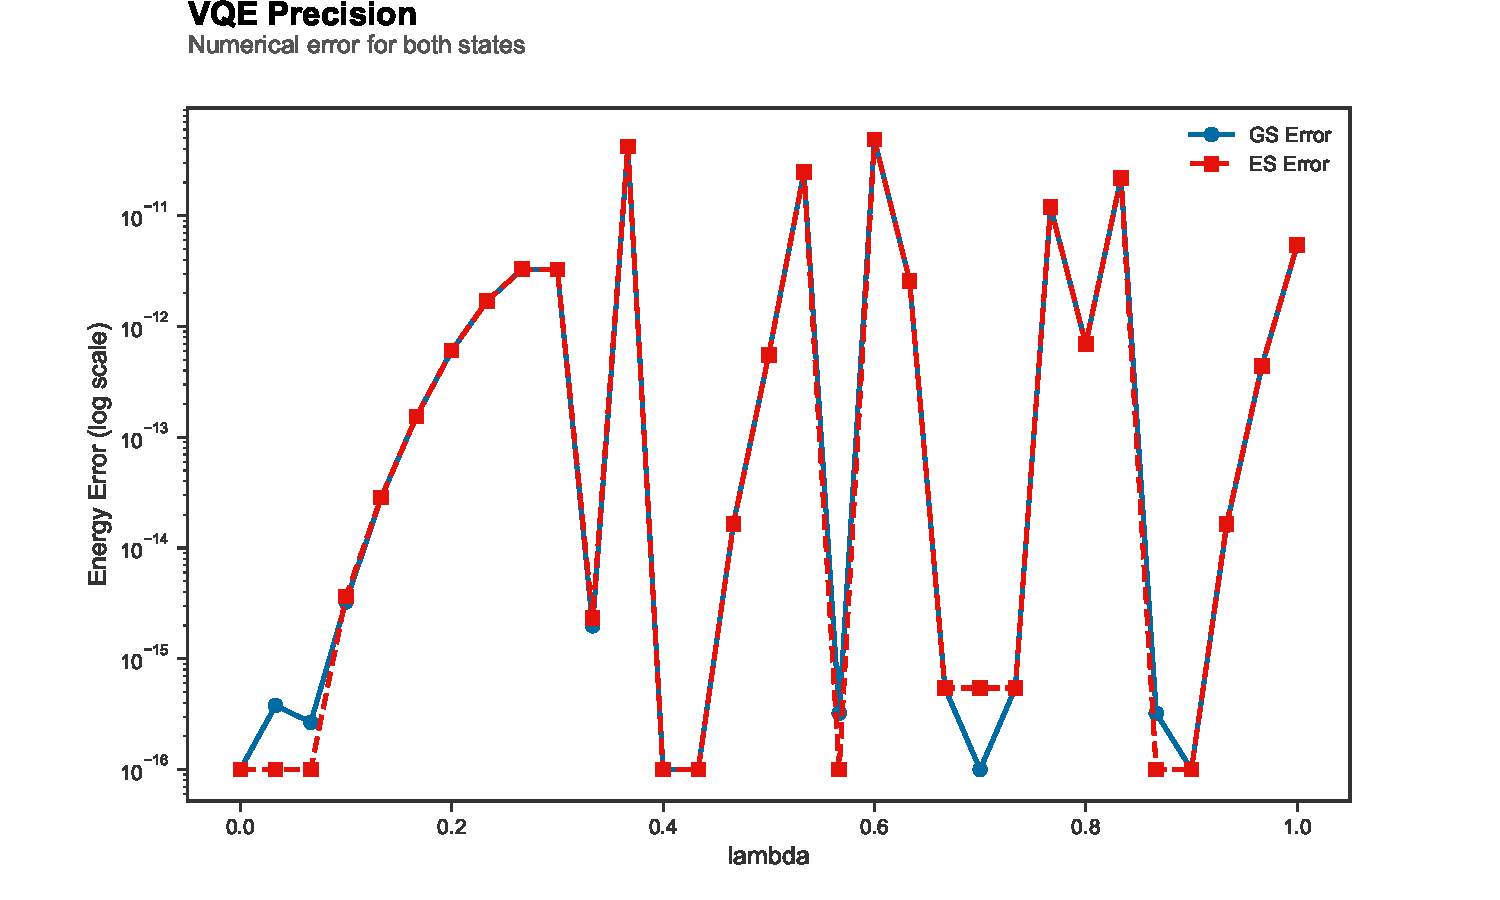
\includegraphics[width=\linewidth]{figures/part-c_vqe_spectrum_error.pdf}
    \caption{Absolute error between the VQE energy and exact diagonalization as a function of $\lambda$, remaining below $10^{-10}$ across the full range for both ground and excited states.}
    \label{fig:part-c_vqe_spectrum_error}
\end{figure}

As the error remains below $10^{-10}$ across the entire $\lambda$ range, this confirms that (i) the $R_y$ ansatz is exact for this $1$-qubit problem, (ii) the BFGS optimizer converges to the global minimum reliably, and (iii) the one-parameter landscape has no local minima. 

An independent VQE-implementation using \texttt{Qiskit}'s \texttt{SparsePauliOp} and \texttt{Statevector} produces identical results, validating the manual implementation.

\subsection{Two-Qubit System and Interaction-Driven Entanglement}
\label{subsec:two-qubit-entanglement}

The two-qubit Hamiltonian with parameters $H_x=2.0,\space H_z=3.0,\space \epsilon_{00}=0.0,\space \epsilon_{10}=2.5,\space \epsilon_{01}=6.5,\space \epsilon_{11}=7.0$ is diagonalized over $\lambda\in[0,1]$.

\begin{figure}[!htbp]
    \centering
    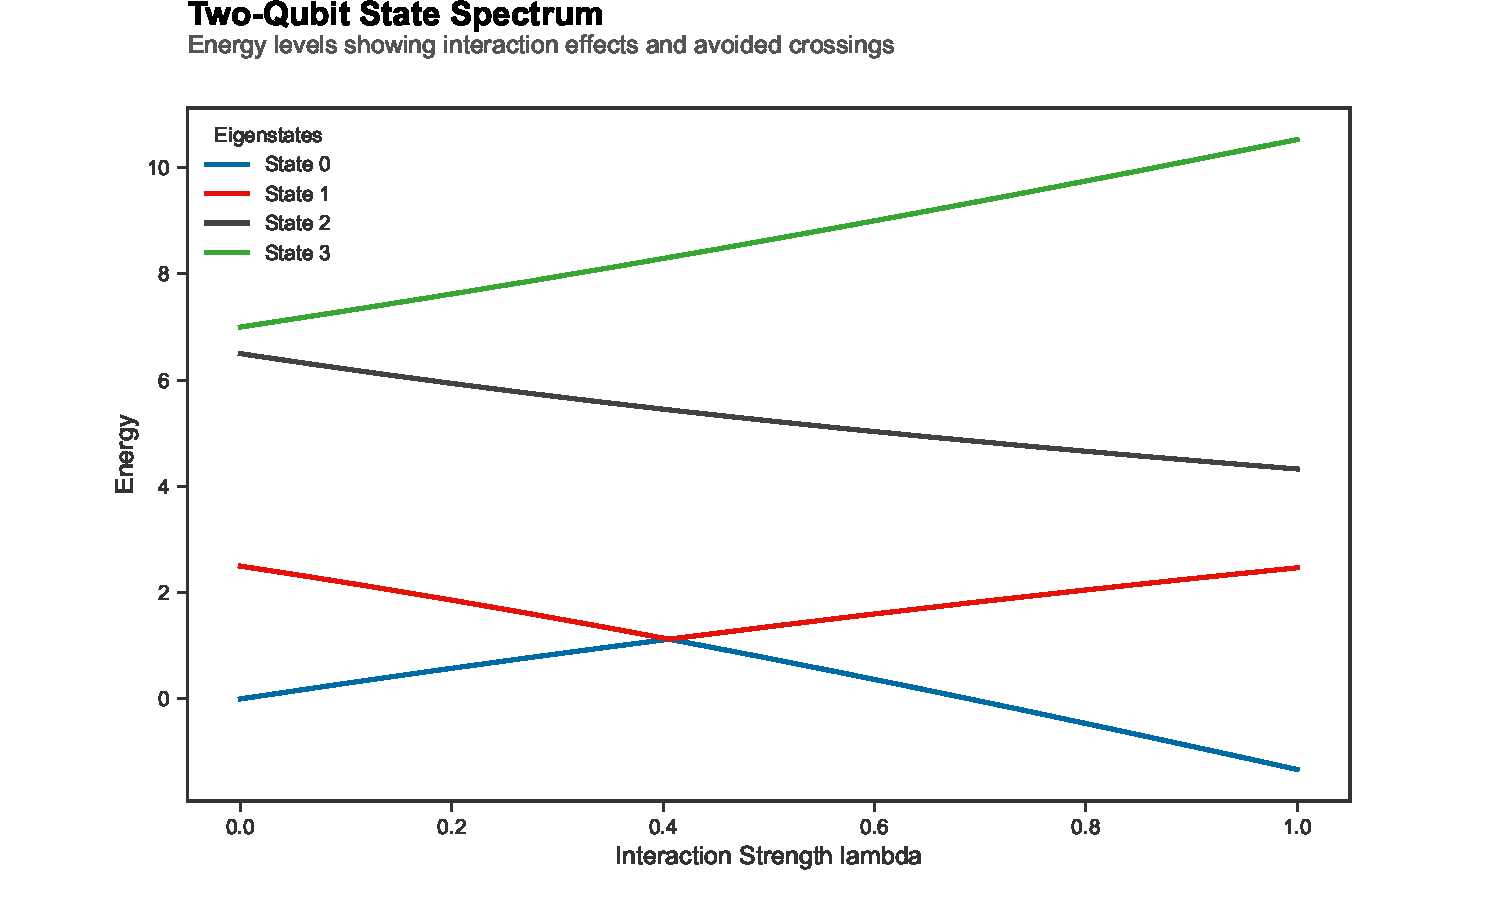
\includegraphics[width=\linewidth]{figures/part-d_eigenvalues.pdf}
    \caption{Eigenvalues of the two-qubit Hamiltonian as a function of $\lambda$, showing pairwise avoided crossings driven by the $\sigma_x\otimes\sigma_x$ coupling.}
    \label{fig:part-d_eigenvalues}
\end{figure}

At $\lambda=0$ the eigenvalues are the non-interacting energies $0.0,\space 2.5,\space 6.5,\space 7.0$. As $\lambda$ increases, the $\sigma_z\otimes\sigma_z$ interaction shifts the diagonal elements, pushing $\ket{00}$ and $\ket{11}$ up while pulling $\ket{10}$ and $\ket{01}$ down. The $\sigma_x\otimes\sigma_x$ coupling then creates off-diagonal mixing between $\ket{00}\leftrightarrow\ket{11}$ and $\ket{01}\leftrightarrow\ket{10}$, producing avoided crossings. The block structure of the Hamiltonian, two independent $2\times2$ blocks, is reflected in the pairwise behaviour of the energy levels.

The von Neumann entropy is computed for all four eigenstates, not just the ground state. 

\begin{figure}[!htbp]
    \centering
    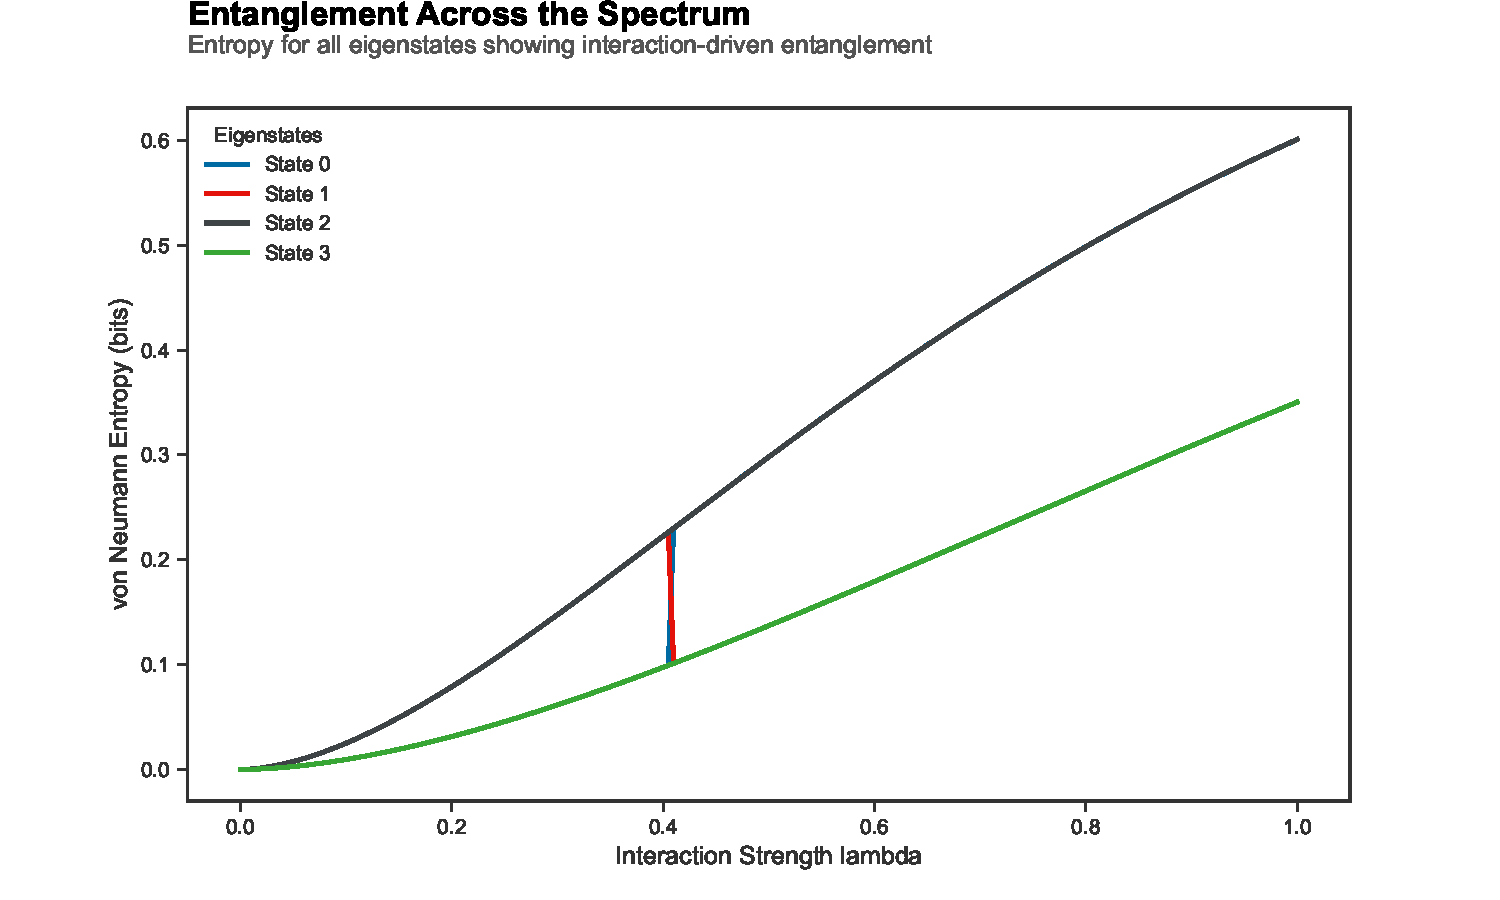
\includegraphics[width=\linewidth]{figures/part-d_entropy.pdf}
    \caption{Von Neumann entropy $\mathcal{S}$ for all four eigenstates as a function of $\lambda$, showing monotonic growth of entanglement with a sharp rise near the avoided crossing.}
    \label{fig:part-d_entropy}
\end{figure}

At $\lambda=0$ all eigenstates coincide with the computational basis states and carry no bipartite correlations, so $\mathcal{S}=0$ exactly. As $\lambda$ grows, the off-diagonal $\sigma_x\otimes\sigma_x$ coupling mixes the basis states within each $2\times2$ block, generating entanglement that increases smoothly with interaction strength.

The most striking feature is the sharp entropy spike near the avoided crossings. At these points the eigenstate character undergoes a rapid transition — the ground state shifts from being dominated by a single product state to being a strongly entangled superposition of two. A small change in $\lambda$ near the crossing therefore produces a disproportionate change in quantum correlations. This is not a numerical artifact; it is a direct consequence of the near-degeneracy at the level repulsion, where the two hybridizing states contribute roughly equally to the eigenstate and maximise the bipartite entropy.

The entanglement is entirely Hamiltonian-driven. It is not imposed externally but emerges from the competition between the diagonal energy spacings $\epsilon_{ij}$ and the off-diagonal coupling $H_x$. When $\lambda H_x$ becomes comparable to the gap between two levels, the corresponding eigenstates can no longer be written as product states and the von Neumann entropy rises sharply. The entropy is therefore a sensitive diagnostic of the balance between single-particle energies and interaction strength, and its peak coincides precisely with the strongest level mixing seen in \cref{fig:part-d_eigenvalues}.

The non-interacting Hamiltonian $\mathcal{H}_0=\text{diag}\left(\epsilon_{00},\space \epsilon_{01},\space \epsilon_{10},\space \epsilon_{11}\right)$ is decomposed into four Pauli strings, as seen in \cref{four-pauli-string}, with $h_0=4.0,\space h_1=-0.75,\space h_2=-2.75,\space h_3=-0.5$. The interaction adds $(h_3+\lambda\mathcal{H}_z),\space ZZ+\lambda\mathcal{H}_x,\space XX$, giving $5$ Pauli terms total.
\begin{equation}\label{four-pauli-string}
    \mathcal{H}_0 = h_0\, II + h_1\, ZI + h_2\, IZ + h_3\, ZZ
\end{equation}

The hardware-efficient ansatz consists of two $R_y$ rotation layers separated by a CNOT entangler shown in \cref{ry-thetha-3} and \cref{fig:circuit-e-1idx}.
\begin{equation}\label{ry-thetha-3}
    \ket{\psi(\theta)} = \left( R_y(\theta_3) \otimes R_y(\theta_4) \right) \cdot \text{CNOT} \cdot \left( R_y(\theta_1) \otimes R_y(\theta_2) \right) \ket{00}
\end{equation}
\begin{figure}[!htbp]
    \centering
    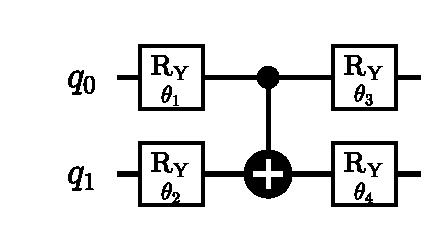
\includegraphics[width=0.55\linewidth]{figures/circuit_part_e_1idx.pdf}
    \caption{Quantum circuit for the two-qubit variational ansatz. The state preparation begins with the qubits in the $\ket{00}$ state. An initial layer of parameterized single-qubit Y-rotations ($R_y(\theta_1)$ and $R_y(\theta_2)$) is applied, followed by an entangling CNOT gate. A final layer of single-qubit Y-rotations ($R_y(\theta_3)$ and $R_y(\theta_4)$) completes the circuit, generating the state $\ket{\psi(\theta)}$}
    \label{fig:circuit-e-1idx}
\end{figure}

This gives $4$ variational parameters. The $R_y$ rotations span the real subspace of each qubit, and the CNOT provides the entanglement needed to represent correlated states. For a $4$-dimensional real Hilbert space, $4$ real parameters are sufficient. 

The VQE sweep over $\lambda\in[0,1]$ compares three approaches in \cref{fig:part-e_vqe_comparison}. For $\lambda\lesssim0.4$ all three curves are indistinguishable, with errors at machine precision as shown in \cref{fig:part-e_vqe_precision}. At $\lambda\approx0.4$ the exact ground state energy reaches a peak of $\approx1.1$ and then drops sharply, falling to $\approx{-1.3}$ at $\lambda=1$. Both VQE implementations, however, continue upward past the crossing, reaching $\approx2.5$ at $\lambda=1$ — the same trajectory as the first excited state.

\begin{figure}[!htbp]
    \centering
    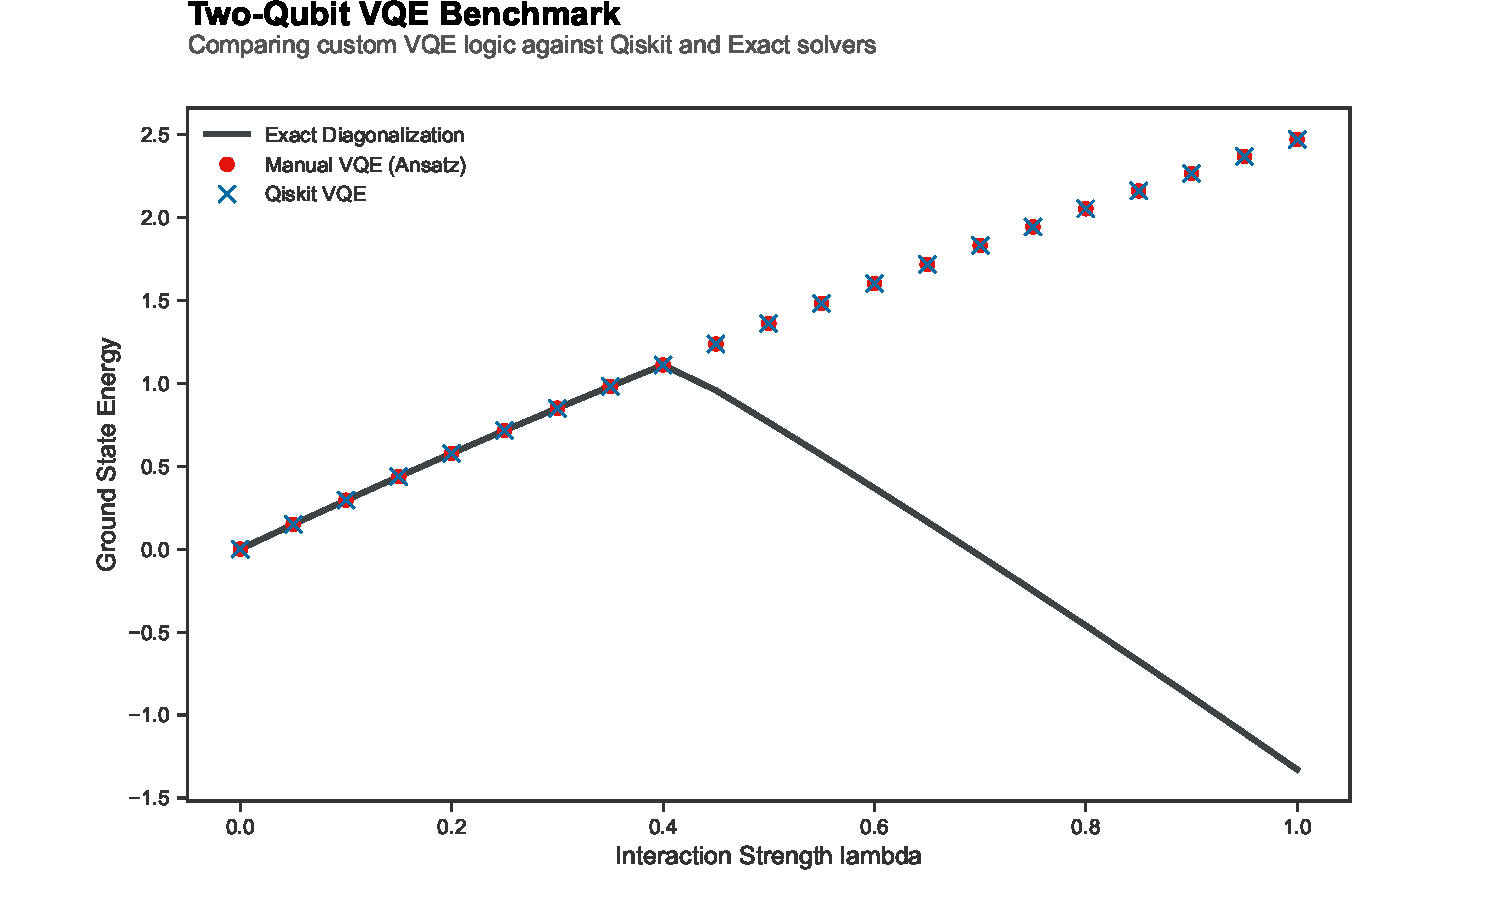
\includegraphics[width=\linewidth]{figures/part-e_vqe_comparison.pdf}
    \caption{Ground state energy as a function of $\lambda$ for three approaches: exact diagonalization, manual VQE, and Qiskit VQE. All three agree for $\lambda\lesssim0.4$. After the avoided crossing at $\lambda\approx0.4$ the exact ground state drops sharply while both VQE methods continue along the upper (excited-state) branch.}
    \label{fig:part-e_vqe_comparison}
\end{figure}

\begin{figure}[!htbp]
    \centering
    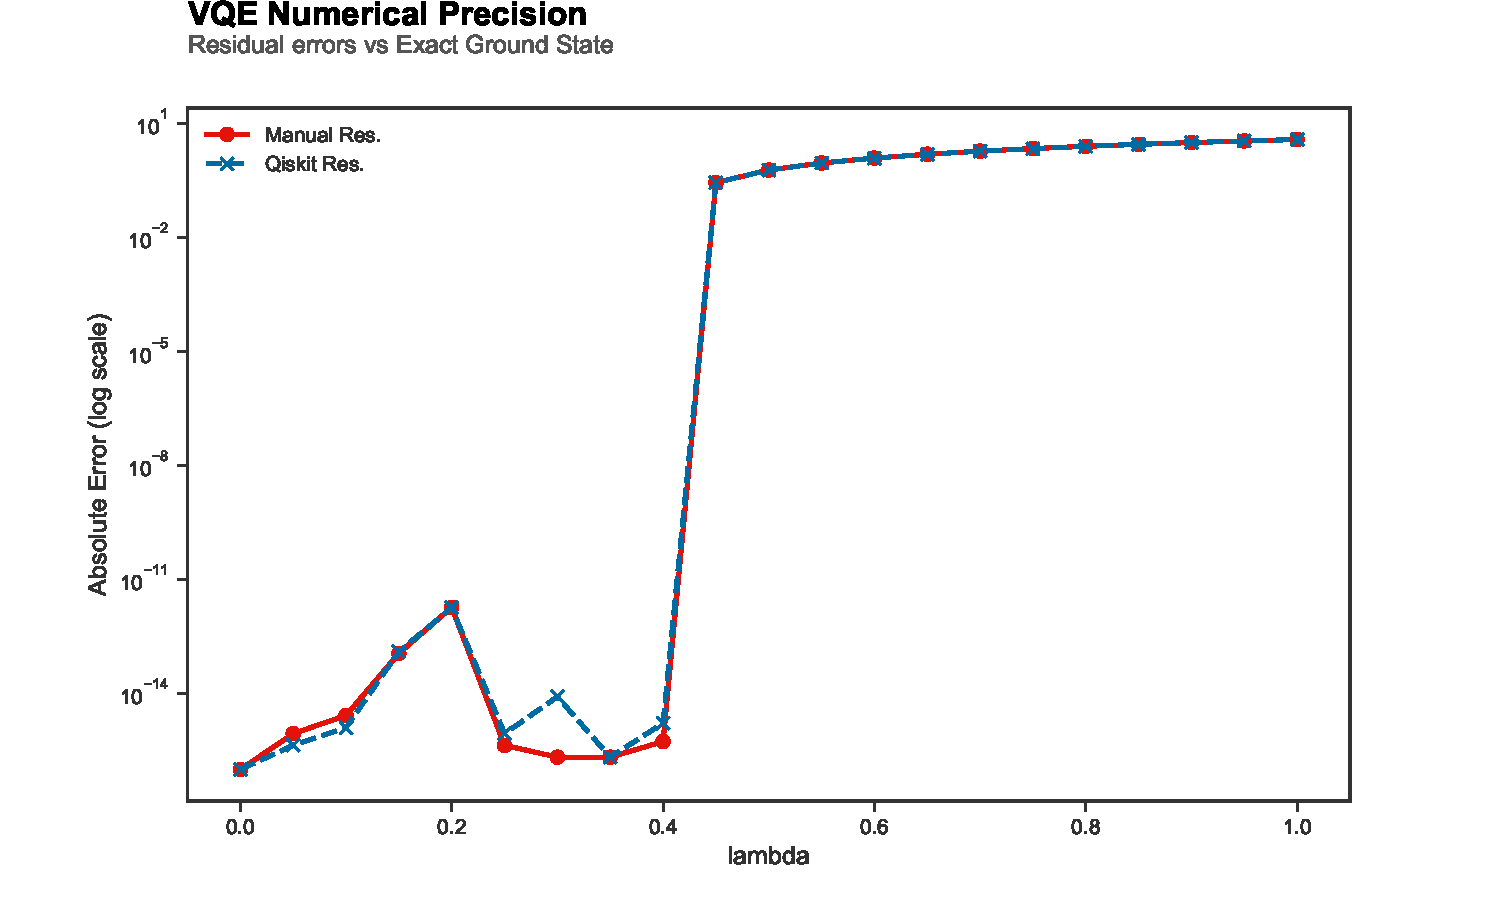
\includegraphics[width=\linewidth]{figures/part-e_vqe_precision.pdf}
    \caption{Absolute error of both VQE implementations relative to exact diagonalization. Below $\lambda\approx0.4$ errors remain at machine precision ($10^{-14}$--$10^{-11}$). At the crossing the error jumps by twelve orders of magnitude and plateaus at $\approx10^{-1}$ for all $\lambda>0.4$, with both implementations failing identically.}
    \label{fig:part-e_vqe_precision}
\end{figure}

The failure is a branch-tracking problem. The $R_y$-CNOT-$R_y$ ansatz is in principle exactly expressive for any real two-qubit state — the ansatz itself is not the limitation. The issue is that BFGS, initialized from $\boldsymbol{\theta}=\mathbf{0}$ at each $\lambda$ value, follows the energy landscape continuously. Before the crossing it finds the true ground state reliably. At the crossing the optimizer has no mechanism to detect that the lower branch has switched character; it stays on the branch it has been tracking, which becomes the first excited state for $\lambda>0.4$.

The fact that both the manual and Qiskit implementations produce identical errors throughout — including in the failure regime — is itself a meaningful result. It rules out a code defect in either implementation and confirms that the breakdown is a systematic consequence of the optimization strategy, not an artifact. Both implementations correctly handle the ansatz, Pauli measurements, and optimization loop; they simply make the same physically motivated mistake at the same crossing point.

For $\lambda\lesssim0.4$, where the VQE does track the ground state, the entanglement structure is correctly captured: as $\lambda$ increases toward the crossing the optimal rotation angles shift so that the CNOT produces increasing entanglement, consistent with the entropy growth in \cref{fig:part-d_entropy}. This correspondence breaks down past the crossing, where the VQE state corresponds to the first excited state rather than the ground state.

\subsection{The Lipkin Model}
\label{subsec:lipkin-model}

The full Lipkin Hamiltonian including both the pair-scattering term ($V$) and the monopole term ($W$) is constructed from the quasispin operators $J_z,\space J_+,\space J_-$. The resulting matrices are shown for $J=1$ with $N=2$ particles ($3\times3$) in \cref{h_j=1_matrix} and $J=2$ with $N=4$ particles ($5\times5$) in \cref{h_j=2_matrix}.

The pair-scattering term $V$ only connects $m \leftrightarrow m\pm2$ states (the $\Delta m = \pm 2$ selection rule from $J_+^2+J_-^2$), so the $m=0$ state is decoupled from the $V$ interaction for all $V$. The $W$ term, however, contributes a diagonal shift: for $J=1$ it raises the $m=0$ energy by $W$, and for $J=2$ it shifts the odd-$m$ states by $3W$ and the $m=0$ state by $4W$, as visible in the matrices below.

\begin{equation}\label{h_j=1_matrix}
    H_{J=1} = \begin{pmatrix}
        -\epsilon & 0 & -V \\
        0 & W & 0 \\
        -V & 0 & \epsilon
    \end{pmatrix}
\end{equation}

The chequerboard pattern $\Delta m = \pm 2$ persists, decoupling even-$m$ and odd-$m$ states into separate blocks.

\begin{equation}\label{h_j=2_matrix}
    H_{J=2} = 
    \begin{pmatrix}
        -2\epsilon & 0 & \sqrt{6}V & 0 & 0 \\
        0 & -\epsilon + 3W & 0 & 3V & 0 \\
        \sqrt{6}V & 0 & 4W & 0 & \sqrt{6}V \\
        0 & 3V & 0 & \epsilon+3W & 0 \\
        0 & 0 & \sqrt{6}V & 0 & 2\epsilon
    \end{pmatrix}
\end{equation}

Mapping the quasispin operators to $N=2$ qubits gives the full two-qubit Hamiltonian
\begin{equation}
    H_{J=1}=\frac{\epsilon}{2}(ZI+IZ)+\frac{V+W}{2}\,XX+\frac{W-V}{2}\,YY
\end{equation}

The $4\times4$ Pauli representation contains both the $J=1$ triplet ($d=3$) and the $J=0$ singlet ($d=1$). Projecting onto the triplet subspace, spanned by $\ket{11}$ $(m=-1)$, $\frac{1}{\sqrt{2}}(\ket{01}+\ket{10})$ $(m=0)$, and $\ket{00}$ $(m=+1)$, exactly reproduces the $3\times3$ quasispin matrix in \cref{h_j=1_matrix}, including the $W$ shift on the $m=0$ diagonal.

For $J=2$, four-qubit mapping:
$$\boxed{H_{J=2} = \frac{\varepsilon}{2}\sum_{i=1}^{4} Z_i + \sum_{i<j}\left(\frac{V+W}{2}\,X_i X_j + \frac{W-V}{2}\,Y_i Y_j\right)}$$

This gives $4$ single-qubit $Z$ terms and $12$ two-qubit interaction terms ($XX$ and $YY$ for each of the $6$ pairs), totalling $16$ Pauli strings regardless of $W$. The $W$ term modifies the coefficients of the existing strings rather than introducing new ones. The $16\times16$ Hilbert space contains $J=0,1,2$ sectors; the five $J=2$ eigenvalues were extracted from the full Pauli spectrum and verified against the quasispin reference at a test point ($\epsilon=1$, $V=0.5$, $W=0.2$).

The primary V-sweeps use $W=0$ as the baseline, and the Pauli decomposition with $W\neq0$ was verified to match the quasispin Hamiltonian exactly for both $J=1$ and $J=2$. Setting $W=0$ recovers the pure pair-scattering model; including $W$ breaks the residual symmetry between the $XX$ and $YY$ channels and lifts the $m=0$ degeneracy seen at $W=0$.

\begin{figure}[!htbp]
    \centering
    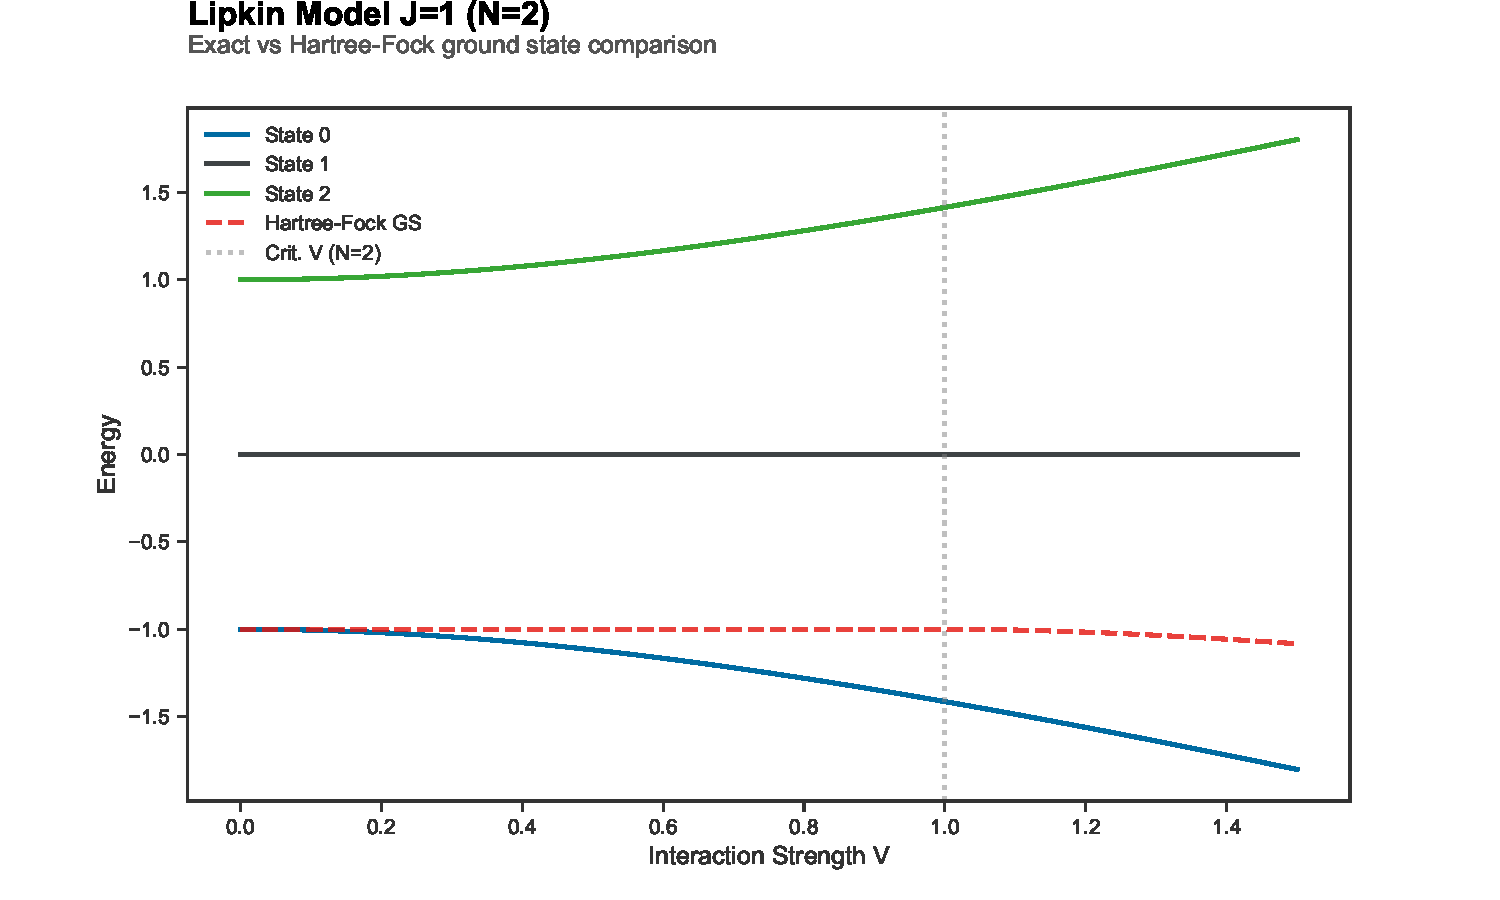
\includegraphics[width=\linewidth]{figures/part-f_j1.pdf}
    \caption{Lipkin model eigenvalues for $J=1$ ($N=2$) as a function of $V$, with $\epsilon=1$ and $W=0$.}
    \label{fig:part-f_j1}
\end{figure}

\begin{figure}[!htbp]
    \centering
    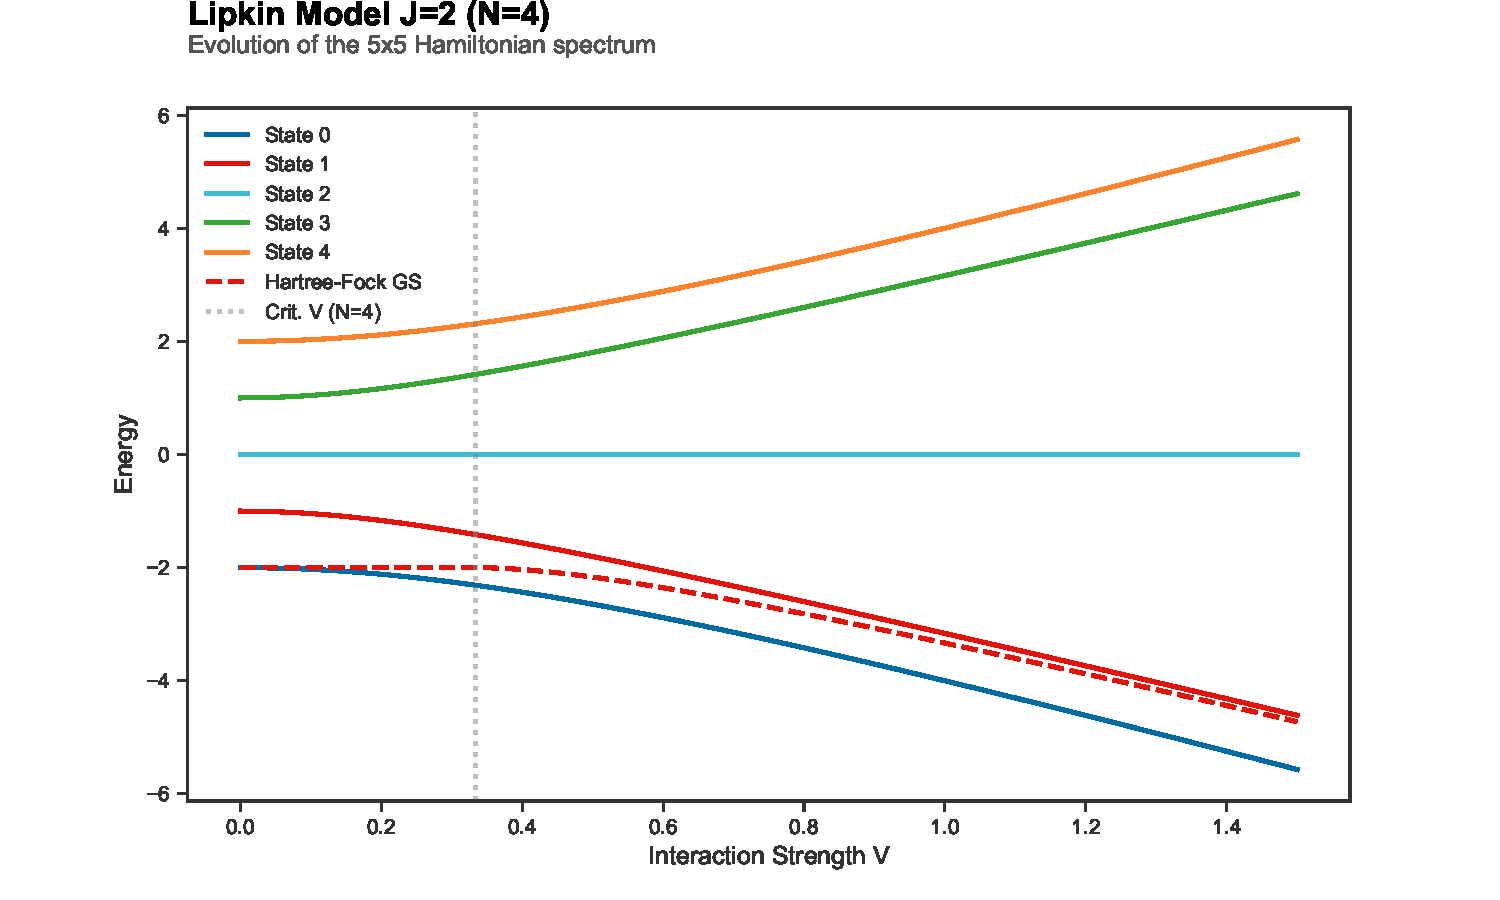
\includegraphics[width=\linewidth]{figures/part-f_j2.pdf}
    \caption{Lipkin model eigenvalues for $J=2$ ($N=4$) as a function of $V$, with $\epsilon=1$ and $W=0$.}
    \label{fig:part-f_j2}
\end{figure}

Both spectra show the ground state energy decreasing with increasing $V$, reflecting energetically favorable pair correlations introduced by the interaction.

The Hartree-Fock energy of the Lipkin model is given in \cref{hartree-fock-energy}, where $\tilde{V}=\frac{(N-1)V}{\epsilon}$, and the critical interaction strengths are $V_c=1.000$ for $N=2$ ($J=1$) and $V_c=0.333$ for $N=4$ ($J=2$).
\begin{equation}\label{hartree-fock-energy}
E_{\text{HF}} = 
\begin{cases}
\frac{-N\epsilon}{2} & \text{if } \tilde{V} \leq 1 \\
\frac{-N\epsilon}{4}\left( \tilde{V}+\frac{1}{\tilde{V}} \right) & \text{if } \tilde{V} > 1 
\end{cases}
\end{equation}

\begin{figure}[!htbp]
    \centering
    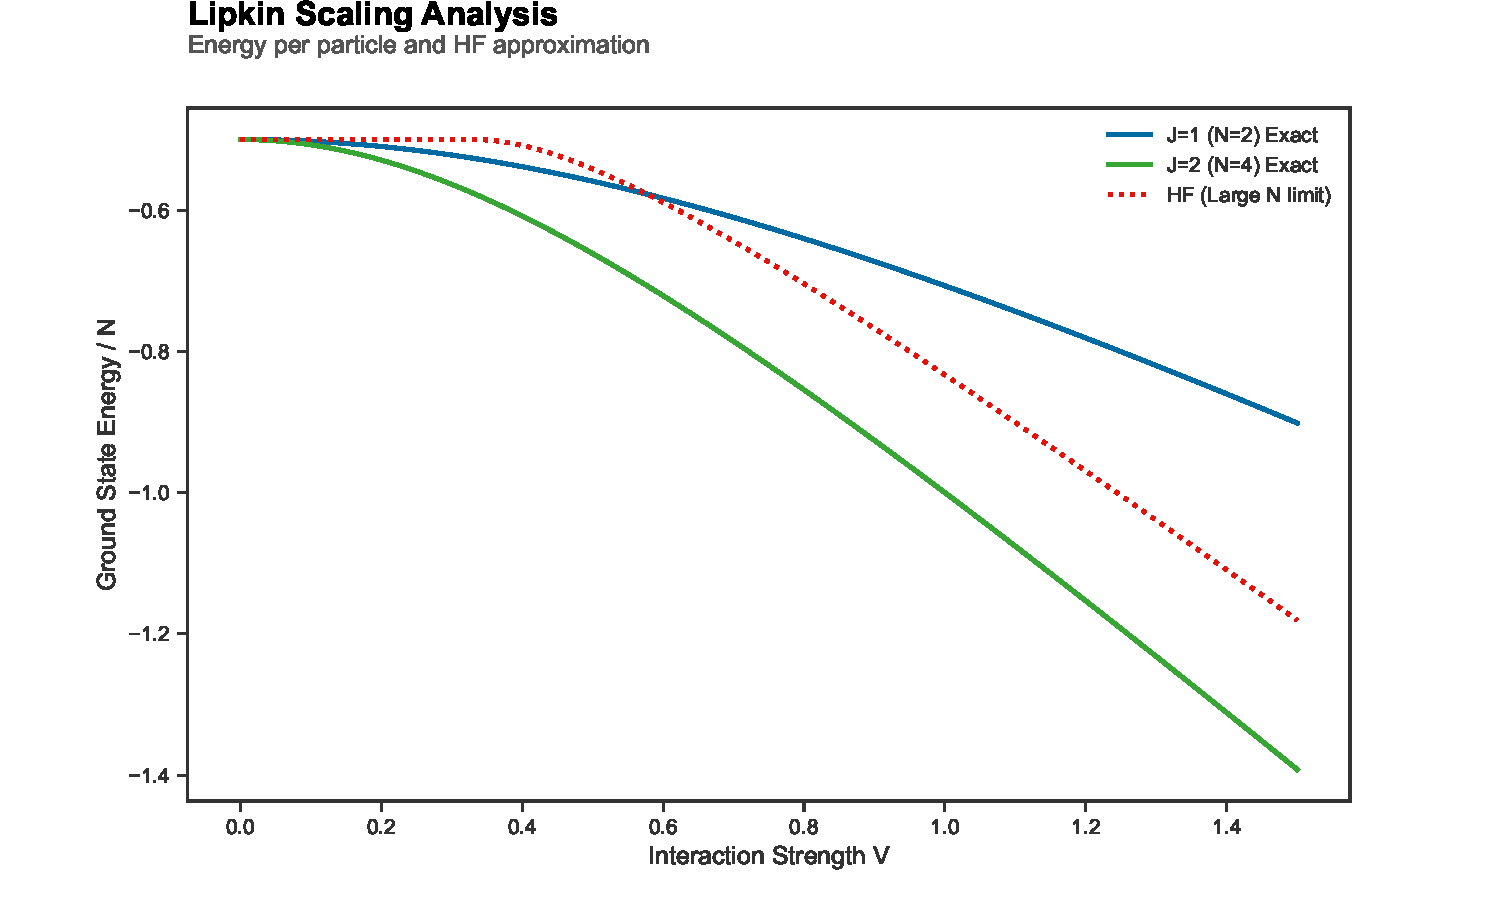
\includegraphics[width=\linewidth]{figures/part-f_scaling.pdf}
    \caption{Ground state energy per particle $E_0/N$ compared with the Hartree-Fock prediction for increasing system sizes, showing convergence of HF to the exact result in the thermodynamic limit.}
    \label{fig:part-f_scaling}
\end{figure}

The energy per particle $\frac{E_0}{N}$ approaches the Hartree-Fock curve as $N$ increases, consistent with HF becoming exact in the thermodynamic limit. Below $V_c$ HF gives the exact answer, the ground state is a single Slater determinant. Above $V_c$ HF systematically overestimates the energy, the correlation energy is missing. 

A hardware-efficient ansatz with $R_y$ rotations and CZ entanglement is used and shown in \cref{tab:vqe-circuit-config}. 

\begin{table}[!htbp]
\centering
\begin{tabular}{cccccc}
\hline
Sys & Qbts & Depth & Params & Restarts & Opt \\
\hline
$J=1$ & 2 & 2 & 4 & 3 & L-BFGS-B \\
$J=2$ & 4 & 4 & 16 & 4 & L-BFGS-B \\
\hline
\end{tabular}
\caption{Variational quantum circuit configurations used for the Lipkin model simulations.}
\label{tab:vqe-circuit-config}
\end{table}

The ansatz uses alternating CZ entanglement layers: even layers entangle pairs $(0,1)$ and $(2,3)$, while odd layers entangle $(1,2)$ and $(3,4)$ plus a wrap-around $(0,3)$ link to ensure full qubit connectivity after two layers. Multiple random restarts mitigate local minima. 
\begin{figure}[!htbp]
    \centering
    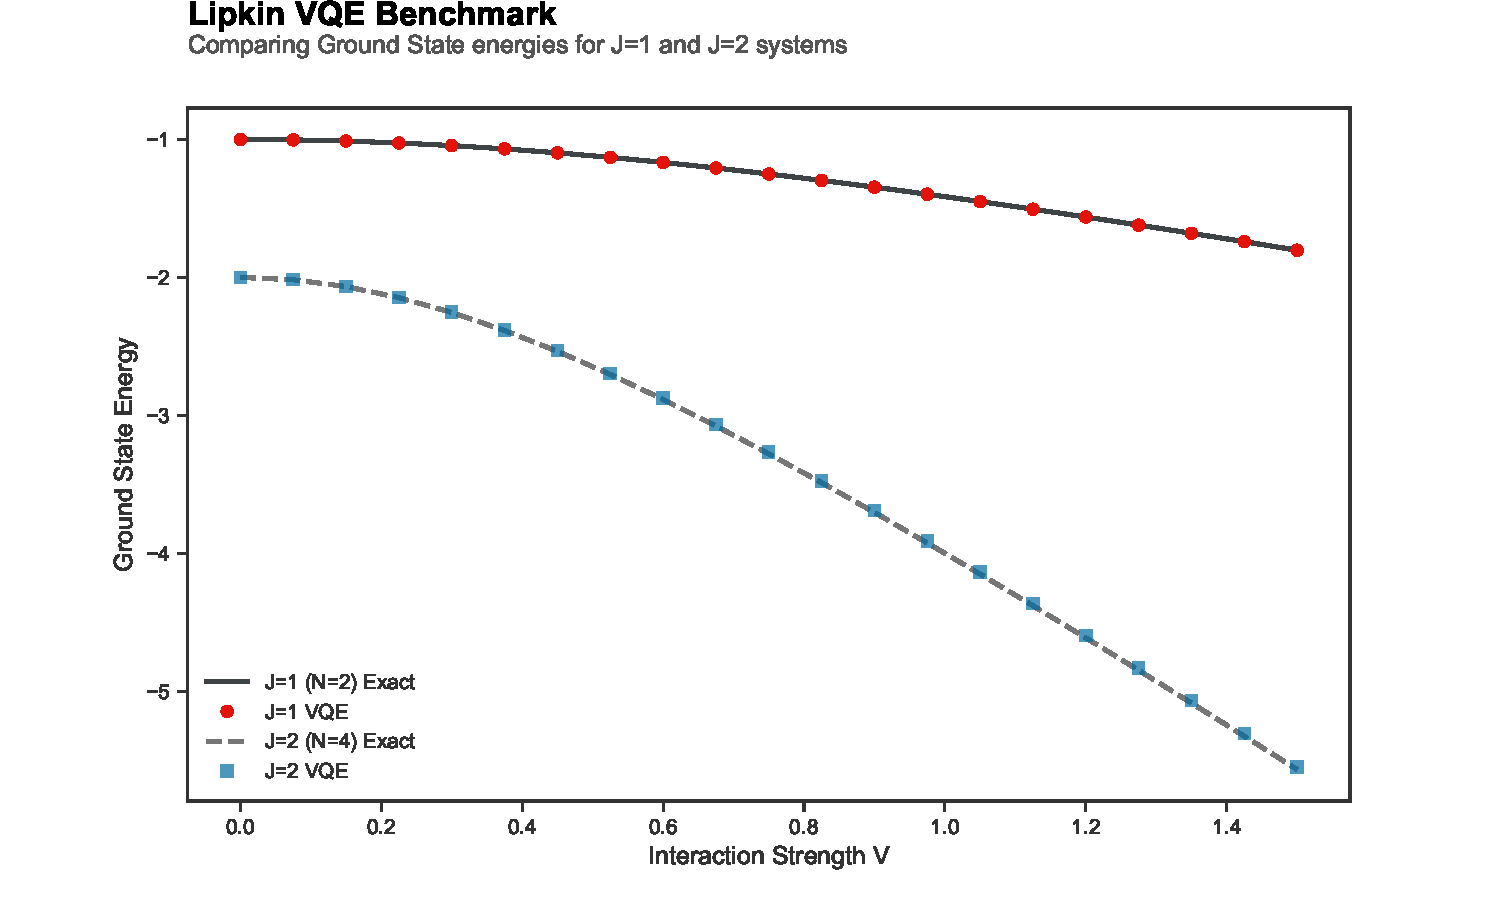
\includegraphics[width=\linewidth]{figures/part-g_vqe_manybody.pdf}
    \caption{VQE ground state energies for both $J=1$ and $J=2$ Lipkin systems compared with exact diagonalization over $V\in[0,1.5]$.}
    \label{fig:part-g_vqe_manybody}
\end{figure}
With this I find a maximum error of $2.92\times10^{-11}$ and $1.80\times10^{-2}$ for $J=1$ ($N=2$) and $J=2$ ($N=4$) respectively, with mean errors of $\approx10^{-12}$ and $\approx10^{-3}$.

For the $J=1$ system, the two-qubit $R_y$-CZ-$R_y$ ansatz achieves near-exact accuracy. The low dimensionality of the problem and the block structure of the Lipkin Hamiltonian mean the variational landscape is smooth, and BFGS converges reliably to the global minimum.
\begin{figure}[!htbp]
    \centering
    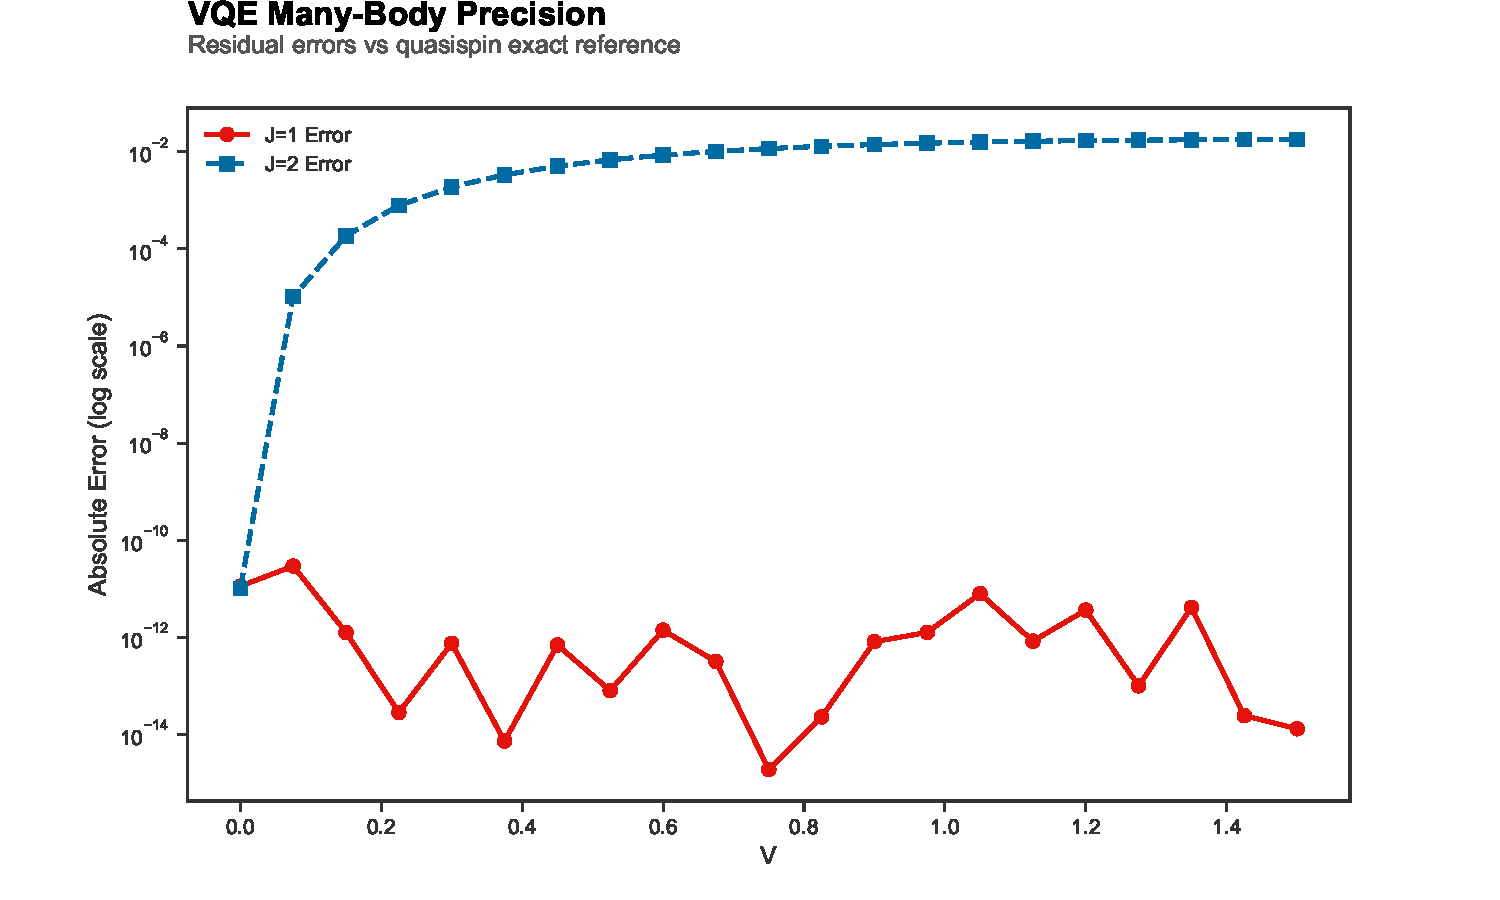
\includegraphics[width=\linewidth]{figures/part-g_vqe_precision.pdf}
    \caption{Absolute VQE error for the Lipkin model. The $J=1$ system achieves machine-precision accuracy ($\approx10^{-11}$), while the $J=2$ system shows a larger residual error ($\approx10^{-2}$) due to the higher-dimensional optimization landscape.}
    \label{fig:part-g_vqe_precision}
\end{figure}
For the $J=2$ system the residual error of $\approx10^{-2}$ is substantially larger and reflects several compounding difficulties. First, the full $16\times16$ qubit Hilbert space contains three symmetry sectors ($J=0,1,2$); the hardware-efficient ansatz imposes no symmetry constraint, so the optimizer must implicitly discover the correct sector from the energy landscape alone. This increases the effective search space and makes convergence to the true $J=2$ ground state less reliable. In practice, the optimized state may be a mixture of sectors or a local minimum in the $J=0$ or $J=1$ region that happens to have a lower apparent energy than the true $J=2$ ground state for some parameter values.

Second, the error is not uniform across the $V$ range: it grows near the phase transition at $V_c\approx0.333$, where the ground state character changes rapidly and the energy landscape becomes flat around the crossing point. Near-flat landscapes cause gradient-based optimizers to stall, leading to poor convergence in exactly the regime of greatest physical interest.

Third, with $16$ parameters and a circuit of depth $4$, the optimization landscape exhibits the signatures of the barren plateau problem \parencite{mcclean2018barren} — gradients of the cost function become exponentially small in regions of parameter space that are far from the solution, making it difficult for gradient-based methods to find a productive direction. The four random restarts partially compensate for this, but they are not sufficient to guarantee global convergence in all cases.

Both systems capture the qualitative behavior of the phase transition: the ground state energy decreases with increasing $V$, and the transition from weak to strong coupling is reflected in a change in the rate of energy decrease. The Hartree-Fock approximation correctly predicts the ground state below the critical coupling but underestimates correlation energy above it, consistent with the scaling analysis in \cref{fig:part-f_scaling}.

The VQE framework scales in qubit count as $N$ for the Lipkin model, but the circuit depth and number of Pauli terms grow as $\mathcal{O}(N^2)$, making it increasingly challenging to maintain precision for large $N$ on near-term hardware.

